\chapter{ТЕОРЕТИЧЕСКАЯ ЧАСТЬ}\label{ch:ch1}

\section{Спутниковые методы позиционирования }\label{sec:ch1/sec1}

В основе спутниковых методов координатных определений находится принцип пространственной линейной засечки, иными словами измерений расстояний от навигационных искусственных спутников Земли (далее «ИСЗ») до определяемого пункта, на котором расположено ГНСС-оборудование.  Расстояния определяются по данным измерения временного ряда прохождения радиосигнала от спутника до приемника.

\subsection{Относительные методы спутникового позиционирования}\label{subsec:ch1/sec1/sub1}

Благодаря использованию относительных методов спутникового позиционирования, существует возможность определения координат с сантиметровыми и субсантиметровыми точностями (характеристиками точности), в зависимости от диапазона расстояний \cite{src01,src09}.

Основной целью относительных спутниковых методов является определение не координат пунктов, а нахождение приращений между ними. В отличие от абсолютных методов спутниковых координатных определений происходит составление фазовых разностей, в следствии чего уменьшается влияние различных задержек.

На рисунке \cref{fig:pic01} приведена общая схема спутникового позиционирования относительным методом.

\begin{figure}[h]
	\centering
	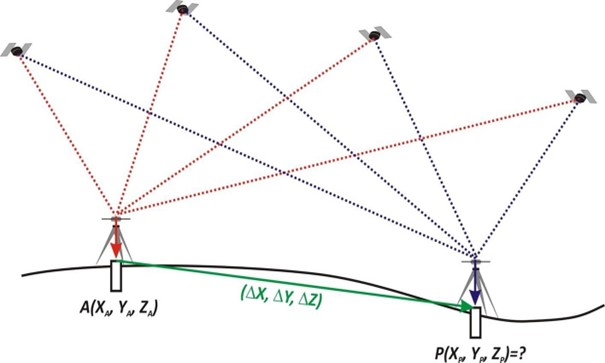
\includegraphics[width=0.7\linewidth]{images/pic01}
	\caption{Относительный метод определения координат}
	\label{fig:pic01}
\end{figure}

На сегодняшний день существует две подгруппы относительных методов: дифференциальные и разностные. 

Для реализации дифференциального подхода необходима хотя бы одна базовая станция, для создания поля поправок, используемых подвижными спутниковыми приемниками --- роверами. При этом корректирующая информация используется в режиме реального времени.

Для реализации разностного подхода необходимо как минимум два спутниковых приемника, запущенных одновременно, тем самым выполняя синхронные измерения. На сегодняшний день существует три способа производства измерений данным методом \cite{src12, src21, src45}: 
\begin{enumerate}[beginpenalty=10000] % https://tex.stackexchange.com/a/476052/104425
	\item Метод вычисления псевдодальностей по измерениям кода сигналов ГНСС (DGPS, DGNSS). Суть метода --- использование кодовой корректирующей информации от дифференциальных (базовых) станций в реальном времени. Точность метода $\thickapprox\nicefrac{1}{2}$ метра. 
	\item Метод с вычислением псевдодальностей по измерениям фазы несущей сигналов ГНСС (Real Time Kinematic (RTK)). Точность определения составляет до 5 сантиметров. 
	\item Сетевой метод определения псевдодальностей по фазе несущей (Network RTK). Суть метода --- применение интегрированной спутниковой корректирующей информации в реальном времени.
\end{enumerate}

На сегодняшний день относительные методы позиционирования с использованием фазовых методов принято делить на \textbf{\textit{статические}} и \textbf{\textit{кинематические}} \cite{src02, src10, src16}.

%\subsubsection{Статические методы}
\textbf{Статические методы}

\textbf{\textit{Статика (Static)}}. Для реализации необходимы синхронные измерения на двух и более пунктах. Один из приемников принимают за базовый, а положение остальных пунктов определяют относительного базового (исходного).

\textit{Относительные методы позиционирования} применяют для определения взаимного положения исходного пункта и определяемого объекта с сантиметровой и более высокой точностью в зависимости от используемого метода позиционирования.

\textbf{\textit{Кинематические методы}}, относящиеся к относительным методам спутникового позиционирования:

\textbf{\textit{Кинематика (kinematic mode)}} --- служит для определения координат передвижной станции в ходе её перемещения. При работе необходимо, чтобы между приемниками, расположенными на базовой станции и подвижным приемником (далее «ровером») поддерживался непрерывный сигнал со спутниками в течении всего времени измерения.

\textbf{\textit{Stop and go}} --- разновидность кинематики. В основе данного метода лежит принцип перемещения ровера, делая на каждой точке движения остановку, продолжительностью от 5 до 30 секунд. На каждой точке для повышения точности измерений принято выполнять измерения с интервалом в несколько эпох.

\textbf{\textit{Непрерывная кинематика (Continuous kinematic)}} --- разновидность кинематики \cite{src02}. Как правило, данный метод измерений происходит в течении одного сеанса с использованием подвижного приемника (ровера) с последующей постобработкой данных.

\textbf{\textit{Технология вычисления координат в режиме реального времени, базирующая на постобработке данных (Real Time Post processesed Kinematic: RTPK)}} --- один из инновационных кинематических методов. Данная технология была разработана основателем компании JAVAD GNNS в 2020 году. По последним сведениям этот режим должен был быть запатентован в США в 2021 году \cite{src73}. Обработку данных можно осуществлять в три этапа: 
\begin{enumerate}
	\item Получение данных с использованием режима измерений RTK.
	\item Постобработка с использованием только ГНСС приемника.
	\item Выполнение верификации(проверки) фиксированного решения.
\end{enumerate}


При использовании данного метода все ГНСС сигналы обрабатываются совместно, что позволяет обеспечить максимально точное нахождение PDOP. Верификация целочисленного решения проводится внутри оригинального алгоритма обработки коварационный матрицы плавающего решения путем сопоставления так называемых частичных решений еще на этапе обработки ковариационной матрицы \cite{src40,src49}. Достоверность этого метода координат выше, чем при использовании метода RTK. В настоящее время режим RTPK реализован в двух версиях программного обеспечения для полевых работ:
\begin{enumerate}
	\item ПО F-Field (доступно в контроллерах Victor-LS и ГНСС приемниках Triumph-LS) 
	\item ПО Javad Mobile Tools – реализовано в контроллерах с операционной системой Android. 
\end{enumerate}

Значения среднеквадратических погрешностей (далее «СКП») определения положения при использовании относительных методов позиционирования можно рассчитать по формуле~\cref{eq:eq1.1}:
\begin{equation}
	\label{eq:eq1.1}
	m=a+bD,
\end{equation}
где: 
\begin{description}
	\item[$m$] -- средняя квадратическая погрешность;
	\item[$D$] -- расстояние между базовым приемником и ровером, в километрах; 
	\item[$a, b$] -- параметры, зависящие от методов спутникового позиционирования и от приемника, приводятся в миллиметрах.
\end{description}



\subsection{Абсолютные методы спутникового позиционирования}\label{subsec:ch1/sec1/sub2}

Автономный метод (navigation mode) --- в основе лежит пространственная линейная засечка. Реализуется по измерениям кода сигналов ГНСС и вычислениям псевдодальностей до спутников.

Метод с использованием поправок к эфемеридно-временной информации, поправок для исключения атмосферных искажений сигнала, поправок к навигационным параметрам (кодовые измерения). Данный метод реализуется с использованием широкозонных систем дифференциальной коррекции ГНСС (Wide area differentinal GNSS).

Метод с использованием поправок в эфемеридо-временной информации, поправок для исключения атмосферных искажений сигналов ГНСС, поправок к навигационным параметрам, измеряемым потребителем (фазовые измерения) – Precise Point Positioning (PPP) \cite{src04, src42, src50}. Данный метод реализуется с использованием глобальных систем дифференциальной коррекции функциональных дополнений ГНСС. Точность зависит от способа обработки и от объема выборки исходных данных. Подробнее о РРР-методах описано в пункте \cref{sec:ch1/sec2}.

На рисунке \cref{fig:pic02} изображен принцип работы абсолютных методов определения координат.
\begin{figure}[h]
	\centering
	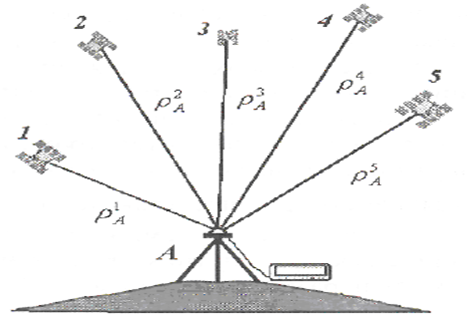
\includegraphics[width=0.7\linewidth]{images/pic02}
	\caption{Принцип работы абсолютных методов}
	\label{fig:pic02}
\end{figure}

Основным параметров, по которому находятся координаты является псевдодальность можно рассчитать по формуле \cref{eq:eq1.2}:
\begin{equation}
	\label{eq:eq1.2}
	P^i_A=r^i_A+c\,dt_A-c\,dt'+I^i_A+T^i_A+d_A+d^i+d\,m^i_A+e^i_A,
\end{equation}
где: 
\begin{description}
	\item[$r^i_A$] -- геометрическая дальность; 
	\item[$dt_A$] -- поправка часов приемника;  $dt'$ -- поправка часов спутника;
	\item[$I^i_A$] -- ионосферная задержка;  $T^i_A$ -- тропосферная задержка;
	\item[$d_A$] -- задержка сигнала приемника;  $d^i$ -- задержка сигнала спутника;
	\item[$d\,m^i_A$] -- влияние многопутности (многолучевости); 
	\item[$e^i_A$] -- случайная ошибка измерений(шум);
	\item[$c$] -- скорость распространения радиоволн в вакууме.
\end{description}



\section{Методы высокоточных координатных определений (PPP) }\label{sec:ch1/sec2}

Метод точного позиционирования (далее «РРР») становится все более востребованным для решения геодезических задач. Используя точные координаты спутников, точное время и многочастотные СРНС метод обеспечивает автономное определение координат с сантиметровой и субсантиметровой точностью. Метод РРР требует меньшего количества опорных пунктов глобального распределения в сравнении с RTK. Единый набор точных эфемерид и поправок часов спутников, получаемый обрабатывающим центром глобальной службы ГНСС доступен для любого пользователя в любой момент времени. Для этого необходим доступ в интернет. Получаемые поправки практически не подвержены влиянию ошибок конкретных опорных станций. Всегда имеется достаточно большое количество опорных станций, наблюдающих одни и те же спутники, так как точные орбиты и поправки часов получают по наблюдениям в глобальной сети станции. За счет этого Методы высокоточных координатных определений обеспечивают получение достаточно устойчивых значений координат и с высокой избыточностью \cite{src74,src75,src76,src77}. 

РРР-алгоритм использует как фазовые, так и кодовые наблюдения многочастотным СРНС приемником, а также эфемериды и поправки часов спутника для вычисления точных координат и поправок часов. При этом, как например, в статике, используются не фазовые разности, а ионосферно-свободная комбинация. Используя её, удается сократить влияние ионосферных явлений вплоть до 99.9\%. При этом кодовая ионосферно-свободная комбинация позволяет корректировать часы спутников.

Наблюдения, принятые со спутников, обрабатываются совместно с использованием процедуры фильтрации, чтобы определить неизвестные значения координат и поправок часов приемника, зенитной тропосферной задержки и фазовых неоднозначностей из решения полученной переопределенной системы уравниваний принимая точные эфемериды за исходные величины.

На сегодняшний день методы высокоточных координатных определений (Precise Point Positioning) можно разделить на три обобщенные группы:
\begin{description}
	\item[PPP (Float PPP)] реализация метода без разрешения целочисленной неоднозначности псевдофазовых измерений.
	\item[РРР-AR (Interger PPP)] с разрешением целочисленной неоднозначности псевдофазовых измерений.
	\item[РРР-RTK] с разрешением целочисленной неоднозначности псевдофазовых измерений и использованием атмосферных коррекций в пределах локальной области.
\end{description}

Для точного определения пространственного положения точки методом РРР используется ионосферно-свободная комбинация двух несущих частот \cite{src03,src05,src12,src19}. 

Стандартная модель измерений соответствует высокоточной эфемеридно-временной информации (далее «ЭВИ») и представлена в виде формулы \cref{eq:eq1.3} на примере комбинации приемник-спутник:
\begin{equation}
	\label{eq:eq1.3}
	\begin{array}{l}
		P_{A}^{i}=\rho+c\left(dt-dT\right)+Tr+\varepsilon_{p}\\
		\varPhi_{if}=\rho+c\left(dt-dT\right)+Tr+N\varLambda+\varepsilon_{\Phi},
	\end{array}
\end{equation}
где: 
\begin{description}
	\item[$\varPhi_{if}, P_{A}^{i}$] -- ионосферная комбинация несущих фаз (L1, L2) и псевдодальностей $(P_1, P_2)$; 
	\item[$dt, dT$] -- ошибка часов приемника и спутника, так называемый сдвиг шкал относительно системной шкалы времени (далее «СШВ»);
	\item[$c$] -- скорость распространения радиоволн в вакууме;
	\item[$Tr$] -- тропосферная задержка;
	\item[$N$] -- целочисленные колебания несущей фазы;  
	\item[$\varLambda$] -- длина несущей волны;
	\item[$\varepsilon_{p}, \varepsilon_{\Phi}$] -- различные шумовые компоненты, включающие многолучевость (многопутность); 
	\item[$\rho$] -- расстояние между спутником и приемником.
\end{description}

На рисунке \cref{fig:pic03} изображена обобщенная схема РРР-метода.
\begin{figure}[h]
	\centering
	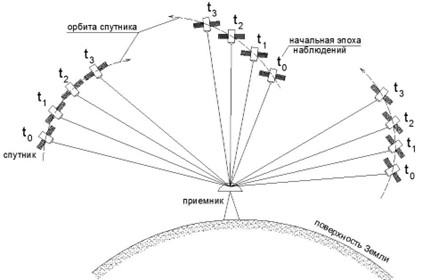
\includegraphics[width=0.7\linewidth]{images/pic03}
	\caption{Cхема РРР-метода}
	\label{fig:pic03}
\end{figure}


\subsection{PPP-AR (Interger PPP)}\label{subsec:ch1/sec2/sub1}

РРР-AR --- Метод высокоточных координатных определений с разрешением целочисленной неоднозначности фазовых измерений.

Для реализации метода PPP-АR необходима спутниковая корректирующая информация, состоящая из поправок к эфемеридам орбит и времени бортовых часов спутников. В дополнении к этому требуются поправки, устраняющие нецелочисленные решения. Все эти поправки формируются сервисами высокоточных спутниковых определений \cite{src41}.  Время получения решения обусловлено временем его сходимости в процессе приема и обработки поступающей ЭВИ. Так, например, для Interger PPP около 10 минут \cite{src54,src57}.

\subsection{PPP-float (float PPP)}\label{subsec:ch1/sec2/sub2}

В данном методе не происходит разрешения целочисленной неоднозначности псевдофазовых измерений. Для реализации метода PPP-float необходима спутниковая корректирующая информация, состоящая из поправок эфемеридам орбит и времени бортовых часов спутников. Время получения решения обусловлено временем его сходимости в процессе приема и обработки поступающей ЭВИ. Так, например, для Float PPP несколько десятков минут \cite{src53,src57,src66}.

\subsection{PPP-RTK}\label{subsec:ch1/sec2/sub3}

PPP-RTK – метод высокоточного абсолютного определения местоположения с разрешением целочисленной неоднозначности псевдофазовых измерений и использованием атмосферных коррекций в пределах локальной области \cite{src68,src71}. 

Кинематика в реальном времени позволяет получить поправки к разрешению целочисленной неоднозначности псевдофазовых измерений, а PPP к эфемеридно-временной информации. PPP-RTK реализуется через поток поправок в формате RTCM-SSR (State Space Representation) \cite{src78,src79}. При этом обеспечивается точность такая же как в методе PPP-AR (Integer PPP). 




\section{Источники погрешностей определения координат}\label{sec:ch1/sec3}

\subsection{Эфемеридно-временная информация}\label{subsec:ch1/sec3/sub1}

Действительное положение спутника при движении по орбите отличается от расчетного в связи с различными возмущающими факторами, оказывающими влияние на скорость и траекторию его движения: лунная и солнечная гравитация, неравномерность гравитационного поля Земли (далее «ГПЗ»), давление излучения Солнца и иные факторы. Вся информация о положении спутника на орбите содержится в эфемеридах \cite{src08,src18,src33}.

Бортовая(стандартная) эфемеридно-временная информация (далее «ЭВИ»), содержащиеся в навигационном сообщении, обеспечивает точность определения положения спутника на орбите с точностью 1--3 метра. Для успешной реализации РРР-метода необходимы высокоточные эфемериды, предоставляемые Международной службой ГНСС (далее «IGS») \cite{src32}.

Помимо точных эфемерид, IGS предоставляет точную информацию о поправках часов каждого спутника относительно системной шкалы времени. Ввиду того, что в ГНСС время также является измеряемой величиной, ошибки шкал времени спутника и приемника являются неотъемлемыми составляющими обработки результатов наблюдений \cite{src35}.

Самые «быстрые» (предрасчитанные) эфемериды (Ultra-Rapid) предоставляется в режиме реального времени, и точность определения положения в этом случае в режиме реального времени достигает точности первых метров и в течение часа наблюдений может быть повышена до дециметровой.

Применение окончательных (Final) эфемерид для обработки результатов суточных наблюдений позволяют достигать максимальной точности, однако для их вычисления IGS требуется произвести обработку большого объема данных, поступающих с сотен постоянно действующих базовых станций.

В таблице \cref{tab:tab01} приведено сравнение различных видов эфемерид между собой, а также сроки предоставления уточненных эфемерид.

\begin{table} [htbp]
	\small
	\centering
	\begin{threeparttable}% выравнивание подписи по границам таблицы
		\caption{Сроки и точность предоставления уточненных эфемерид\tablefootnote{Примечание к таблице. $RMS$~--- в данном случае это СКО без учета аппаратурных задержек, $SDev$~--- СКО с учетом удаления отдельных смещений для каждого тактового сигнала спутника и приемника.}}\label{tab:tab01}%
\begin{tabular}{|cc|c|c|c|}
	\hline
	\multicolumn{2}{|c|}{\textbf{Тип}}                                                                                                                                                                                      & \textbf{Точность}                                                           & \textbf{Задержка}                                                          & \textbf{\begin{tabular}[c]{@{}c@{}}Стандартный \\ интервал\end{tabular}}  \\ \hline
	\multicolumn{2}{|c|}{1}                                                                                                                                                                                                 & 2                                                                           & 3                                                                          & 4                                                                         \\ \hline
	\multicolumn{1}{|c|}{\multirow{2}{*}{\begin{tabular}[c]{@{}c@{}}Стандартные\\  (Broadcast)\end{tabular}}}  & орбиты  & $\sim$100 см  & \multirow{2}{*}{\begin{tabular}[c]{@{}c@{}}Реальное \\ время\end{tabular}} & \multirow{2}{*}{ежедневно}                                                \\ \cline{2-3}
	\multicolumn{1}{|c|}{}  & часы спутника                                                       & \begin{tabular}[c]{@{}c@{}}$\sim$5 нс RMS\tnote{1}\\ $\sim$2,5нс SDev\tnote{2}\end{tabular}   &                                                                            &                                                                           \\ \hline
	\multicolumn{1}{|c|}{\multirow{2}{*}{\begin{tabular}[c]{@{}c@{}}Сверхбыстрые \\предвычисленные \\(Ultra-Rapid \\predicted half)\end{tabular}}} & \begin{tabular}[c]{@{}c@{}}~\\орбиты\\~\end{tabular}  & $\sim$5 см  & \multirow{2}{*}{\begin{tabular}[c]{@{}c@{}}Реальное \\ время\end{tabular}} & \multirow{2}{*}{15 мин}                                                   \\ \cline{2-3}
	\multicolumn{1}{|c|}{}                                                                                                                            & часы спутника                                                       & \begin{tabular}[c]{@{}c@{}}$\sim$3 нс RMS\tnote{1}\\ $\sim$1,5нс SDev\tnote{2}\\~\end{tabular}   &                                                                            &                                                                           \\ \hline
	\multicolumn{1}{|c|}{\multirow{2}{*}{\begin{tabular}[c]{@{}c@{}}Сверхбыстрые \\ измеренные \\ (Ultra-Rapid \\ observed half)\end{tabular}}}       & \begin{tabular}[c]{@{}c@{}}~\\орбиты\\~\end{tabular}                 & $\sim$3 см                                                                  & \multirow{2}{*}{3 - 9 часов}                                               & \multirow{2}{*}{15 мин}                                                   \\ \cline{2-3}
	\multicolumn{1}{|c|}{}                                                                                                                            & часы спутника                                                       & \begin{tabular}[c]{@{}c@{}}$\sim$150 пс RMS\tnote{1}\\ $\sim$50 пс SDev\tnote{2}\\~\end{tabular} &                                                                            &                                                                           \\ \hline
	\multicolumn{1}{|c|}{\multirow{2}{*}{Быстрые (Rapid)}}                                                                                            & орбиты                                                              & $\sim$2,5 см                                                                & \multirow{2}{*}{\begin{tabular}[c]{@{}c@{}}17 - 41 \\ часов\end{tabular}}  & 15 мин                                                                    \\ \cline{2-3} \cline{5-5} 
	\multicolumn{1}{|c|}{}                                                                                                                            & \begin{tabular}[c]{@{}c@{}}часы спутника\\ и приемника\end{tabular} & \begin{tabular}[c]{@{}c@{}}$\sim$75 пс RMS\tnote{1}\\ $\sim$25 пс SDev\tnote{2}\end{tabular}  &                                                                            & 5 мин                                                                     \\ \hline
	\multicolumn{1}{|c|}{\multirow{2}{*}{\begin{tabular}[c]{@{}c@{}}Окончательные \\ (Final)\end{tabular}}}                                           & орбиты                                                              & $\sim$2,5 см                                                                & \multirow{2}{*}{\begin{tabular}[c]{@{}c@{}}12 - 18 \\ суток\end{tabular}}  & 15 мин                                                                    \\ \cline{2-3} \cline{5-5} 
	\multicolumn{1}{|c|}{}                                                                                                                            & \begin{tabular}[c]{@{}c@{}}часы спутника\\ и приемника\end{tabular} & \begin{tabular}[c]{@{}c@{}}$\sim$75 пс RMS\tnote{1}\\ $\sim$20 пс SDev\tnote{2}\end{tabular}  &                                                                            & \begin{tabular}[c]{@{}c@{}}спутник: 30с\\ приемник: \\ 5 мин\end{tabular} \\ \hline
	\end{tabular}  
	\begin{tablenotes}
		\item [1] RMS~--- в данном случае это СКО без учета аппаратурных задержек, 
		\item [2] SDev~--- СКО с учетом удаления отдельных смещений для каждого тактового сигнала спутника и приемника.
	\end{tablenotes}
	\end{threeparttable}
\end{table}



\subsection{Релятивистские поправки}\label{subsec:ch1/sec3/sub2}

Релятивистская поправка часов спутника зависит от положения и скорости движения спутника по орбите \cite{src38, src39} и определяется по формуле \cref{eq:eq1.4}:
\begin{equation}
	\label{eq:eq1.4}
	\Delta t_{rel}^{sat}=\frac{2\overrightarrow{R}\overrightarrow{V}}{c^{2}}
\end{equation}
где: 
\begin{description}
	\item[$\overrightarrow{R}$] -- мгновенный вектор положения спутника на орбите; 
	\item[$\overrightarrow{V}$] -- мгновенный вектор скорости спутника;
	\item[$c$] -- скорость распространения сигнала в вакууме.
\end{description}

Для определения релятивистской поправки можно воспользоваться формулой \cref{eq:eq1.5}: 
\begin{equation}
	\label{eq:eq1.5}
	\Delta t_{rel}^{sat}=t-\tau\left(t\right)\approx t_{0}-\tau\left(t_{0}\right)-\intop_{t_{0}}^{t}\frac{\Delta W}{c^{2}}\mathrm{d}t,
\end{equation}
где: 
\begin{description}
	\item[$t$] -- текущий момент координатного времени; 
	\item[$\tau\left(t\right)$] -- время приемника на момент времени $t$;
	\item[$t_{0}$] -- начальный момент координатного времени;
	\item[$\Delta W$] -- разность потенциалов силы тяжести на точке установки приемника на момент времени $t$ и потенциала силы тяжести геоида распространения сигнала в вакууме;
	\item[$c$] -- скорость распространения сигнала в вакууме;
	\item[$\mathrm{d}t$] -- ошибка часов приемника.
\end{description}


\subsection{Вариации фазового центра антенны спутника и приемника}\label{subsec:ch1/sec3/sub3}

Как и остальные факторы, смещение фазового центра оказывает влияния на точность определения координат при использовании спутниковых методов координатных определений \cite{src36}. Вариация(смещение) фазового центра антенны приемника зависит от зенитного расстояния и азимута линии приемник~--~спутник, значение данной величины так же меняется в зависимости от типов антенны и распространяется в открытом доступе сервисами IGS в формате ANTEX \cite{src13,mak03,src82}.

Высокоточные эфемериды ГНСС, характеризующие положение спутника на орбите, отнесены к центру масс спутника, в то же время, для сигналов, генерируемых аппаратурой спутника, отправной точкой является фазовый центр передающей антенны \cite{src86,src90}. Местоположение центра масс спутника и фазового центра передающей антенны не совпадают (\cref{fig:pic04a}). Помимо смещения фазового центра антенны относительно цента масс спутника, которая является величиной постоянной, выделяют так же вариацию фазового центра, зависящую от угла надира направления спутник~--~приемник (\cref{fig:pic04b}).

\begin{figure}[ht]
	\centerfloat{
		\hfill
		\subcaptionbox[List-of-Figures entry]{Смещение ЦМ спутника \\и ФЦ антенны\label{fig:pic04a}}{%
			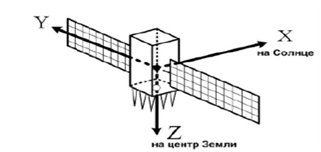
\includegraphics[width=0.45\linewidth]{images/pic04a}}
		\hfill
		\subcaptionbox{Вариация фазового центра\label{fig:pic04b}}{%
			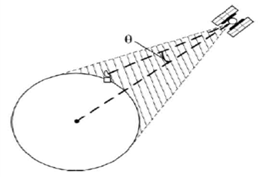
\includegraphics[width=0.45\linewidth]{images/pic04b}}
		\hfill
	}
	\legend{$\bullet-\text{центр масс (ЦМ)}\qquad\circ-\text{фазовый центр (ФЦ)}$\\
		}
	\caption[Расположение фазовых центров]{Расположение фазовых центров}\label{fig:pic04}
\end{figure}

% Подрисуночный текст, описывающий обозначения, например. Согласно ГОСТ 2.105, пункт 4.3.1, располагается перед наименованием рисунка.

\subsection{Тропосферная задержка}\label{subsec:ch1/sec3/sub4}

Для учета влияния тропосферной задержки тропосферу принято разделять на сухую и влажную составляющие.

Сухая составляющая, обусловливается рефракцией сухих газов: азот (78,09\%), кислород (20,95\%), аргон (0,93\%), углекислый газ (0,03\%), а также частью недипольного компонента водяного пара.

Влажная составляющая обусловлена неоднородным распределением водяного пара, связанным с быстрым изменением его агрегатного состояния на поверхности планеты, а также коррелирует с изменениями температуры в зависимости от высоты и местоположения.

Для вычисления тропосферной задержки используют различные модели тропосферы: использующие реальную метеорологическую информацию модель Хопфилд, модель Саастамойнена, модель Блэка и статистические модели, такие как MOPS и GCAT \cite{src48, src61, src62, src70}.

\subsection{Ионосферная задержка}\label{subsec:ch1/sec3/sub5}

Ионосфера располагается на высотах примерно от 50~км над поверхностью Земли и, являясь естественным отражателем для низкочастотных радиоволн, оказывает замедляющее влияние на скорость прохождения высокочастотных. В общем виде ионосферная задержка обратно пропорциональна квадрату частоты сигнала \cite{src05, src06, src13} [5,6,13].

Существует ряд способов учета ионосферной задержки. Один из наиболее надежных и проверенных временем --- модель Клобучара (Klobuchar), параметры которой передаются в навигационном сообщении \cite{src64}. Данная модель позволяет при помощи восьми коэффициентов снизить влияние ионосферной задержки до 50\%, при этом необходимо знать широту и долготу точки наблюдения, а также азимут и зенитное расстояние направления на спутник на момент наблюдения в системе местного времени \cite{src41, src46}.

\subsection{Многолучевость}\label{subsec:ch1/sec3/sub6}

К случайным (шумовым) компонентам следует отнести явление «многолучевости» (multipath) --- переотражения сигнала от подстилающей поверхности или вертикальных преград: стен зданий, ограждений и т.д. Техническим вариантом минимизации влияния переотражения на результаты наблюдений может быть установка принимающей антенны на определенную высоту от подстилающей поверхности (от 1~--~1,5 метров), выбор точки наблюдений как можно дальше от вертикальных преград, использование специальных антенн с применением технологии дроссельных колец (choke ring) (рис. \cref{fig:pic05}), заглушающих сигналы, приходящие со спутников, находящихся близко к горизонту, а так же установки маски угла возвышения (elevation mask) в переделах 10~--~15 градусов \cite{src53}.
\begin{figure}[h]
	\centering
	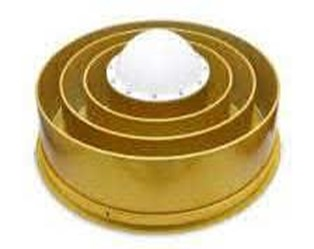
\includegraphics[width=0.7\linewidth]{images/pic05}
	\caption[ГНСС-антенна Choke Ring]{ГНСС-антенна с экраном подавления переотражения сигналов Choke Ring}
	\label{fig:pic05}
\end{figure}



\subsection{Влияние dop-факторов}\label{subsec:ch1/sec3/sub7}

Данный термин принято использовать для геометрического описания местоположения спутников относительно друг друга. Чем дальше расположены спутники, тем ниже значение dop-факторов \cite{src56, src58, src63} [56,58,63]. Среди факторов, влияющих на снижение точности (dop-факторы) можно выделить следующие:
\begin{enumerate}
	\item орбиты спутников;
	\item наличие объектов-помех;
	\item влияние атмосферы;
	\item отражение радиоволн.
\end{enumerate} 

\vspace{5mm}

На основании вышесказанного существует следующая классификация dop-факторов:

\begin{description}
	\item [GDOP (Geometric)] --- полное снижение точности;
	\item [HDOP (Horizontal)] --- снижение точности в горизонтальной плоскости;
	\item [VDOP (Vertical)] --- снижение точности в вертикальной плоскости;
	\item [PDOP (Position)] --- снижение точности по местоположению;
	\item [TDOP (Time)] --- снижение точности по времени.
\end{description}

\vspace{5mm}

В таблице \cref{tab:tab02} приводятся основные численные значения влияния dop факторов на результаты спутниковых координатных определений.




%
%
%\noindent\begin{minipage}{\linewidth}
%	\centering\vspace{5mm}
%	\captionof{table}{Влияние pdop фактора на получаемые результаты}\label{tab:tab02-1}\resizebox{\linewidth}{!}{%
%		\begin{tabular}{|c|c|l|} \hline
%			\textbf{Значение PDOP} & \textbf{Точность} & \multicolumn{1}{c|}{\textbf{Описание}} \\ \hline
%			$<1$ & Идеальная & \begin{tabular}[c]{@{}l@{}}Рекомендуется к использованию в системах, \\требующих максимально возможной точности \\во все время их работы\end{tabular} \\ \hline
%			$2-3$ & Отличная & \begin{tabular}[c]{@{}l@{}}Достаточная точность для использования \\результатов измерений в достаточно \\чувствительной аппаратуре и программах\end{tabular} \\ \hline
%			$4-6$ & Хорошая & \begin{tabular}[c]{@{}l@{}}Рекомендуемый минимум для принятия решений \\по полученным результатам. Результаты могут быть \\использованы для достаточно точных навигационных указаний\end{tabular} \\ \hline
%			$6-8$ & Средняя & \begin{tabular}[c]{@{}l@{}}Результаты можно использовать в вычислениях, \\однако рекомендуется озаботиться повышением точности, \\например, выйти на более открытое место\end{tabular} \\ \hline
%			$9-20$ & Ниже среднего & \begin{tabular}[c]{@{}l@{}}Результаты могут использоваться только \\для грубого определения местоположения\end{tabular} \\ \hline
%			$>20$ & Плохо & \begin{tabular}[c]{@{}l@{}}Результаты даже не могут использоваться \\для грубого определения местоположения\end{tabular} \\ \hline
%		\end{tabular}
%	}
%\end{minipage}
%


\begin{table}[h]
	\small
	\centering\vspace{5mm}
	\begin{threeparttable}% выравнивание подписи по границам таблицы
		\captionof{table}{Влияние pdop фактора на получаемые результаты}\label{tab:tab02}
			\begin{tabular}{|c|c|l|} \hline
			\textbf{\begin{tabular}[c]{@{}c@{}}Значение \\ PDOP\end{tabular}} & \textbf{Точность} & \multicolumn{1}{c|}{\textbf{Описание}} \\ \hline
			$<1$ & Идеальная & \begin{tabular}[c]{@{}l@{}}Рекомендуется к использованию в системах, \\требующих максимально возможной точности \\во все время их работы\end{tabular} \\ \hline
			$2-3$ & Отличная & \begin{tabular}[c]{@{}l@{}}Достаточная точность для использования \\результатов измерений в достаточно \\чувствительной аппаратуре и программах\end{tabular} \\ \hline
			$4-6$ & Хорошая & \begin{tabular}[c]{@{}l@{}}Рекомендуемый минимум для принятия решений \\по полученным результатам. Результаты могут быть \\использованы для достаточно точных навигационных указаний\end{tabular} \\ \hline
			$6-8$ & Средняя & \begin{tabular}[c]{@{}l@{}}Результаты можно использовать в вычислениях, \\однако рекомендуется озаботиться повышением точности, \\например, выйти на более открытое место\end{tabular} \\ \hline
			$9-20$ & \begin{tabular}[c]{@{}c@{}}Ниже \\ среднего\end{tabular}  & \begin{tabular}[c]{@{}l@{}}Результаты могут использоваться только \\для грубого определения местоположения\end{tabular} \\ \hline
			$>20$ & Плохо & \begin{tabular}[c]{@{}l@{}}Результаты даже не могут использоваться \\для грубого определения местоположения\end{tabular} \\ \hline
		\end{tabular}

	\end{threeparttable}
\end{table}

		
%% Нумерованная формула с описанием и примером кроссылки.	 
%\cref{eq:eq_._}
%\begin{equation}
%	\label{eq:eq_._}
%\end{equation}
%где: 
%\begin{description}
%	\item[$ $] --  ; 
%	\item[$ $] --  ;
%	\item[$ $] --  ;
%\end{description}









%\noindent\rule{\textwidth}{1pt}\newpage
%===============================================================================================================================

